\documentclass{article}
\usepackage{graphicx}
\usepackage{listings}
\usepackage{xcolor}
\usepackage{caption}
\usepackage{longtable}
\usepackage{amsmath}
\usepackage{float} 

\title{\textbf{Experiment 2: Loan Amount Prediction using Linear Regression}}
\author{Moogambigai A}
\date{July 2025}

\begin{document}

\maketitle

\section{Aim}
To develop and evaluate a Linear Regression model that predicts the loan sanction amount using historical loan data and relevant borrower features.

\section{Libraries USed}
\begin{itemize}
\item Pandas: Data manipulation

\item NumPy: Numerical operations

\item Scikit-learn: Model building, preprocessing, and evaluation

\item Matplotlib and Seaborn: Data visualization
\end{itemize}


\section{Objective}
\begin{itemize}
    \item Preprocess and clean the dataset

\item Perform exploratory data analysis (EDA)

\item Engineer features to improve model accuracy

\item Train and validate a Linear Regression model

\item Evaluate model performance using MAE, MSE, RMSE, and R² metrics

\item Visualize results and interpret model behavior
\end{itemize}

\section{Mathematical Description}
In this experiment, \textbf{Linear Regression} is used to predict the loan sanction amount based on several input features.

The mathematical model for Linear Regression is:

\begin{equation}
    y = \beta_0 + \beta_1 x_1 + \beta_2 x_2 + \cdots + \beta_n x_n + \epsilon
\end{equation}

Where:

\begin{itemize}
    \item $y$ is the dependent variable (Loan Sanction Amount).
    \item $x_1, x_2, \ldots, x_n$ are the independent variables (features such as Age, Income, Credit Score, etc.).
    \item $\beta_0$ is the intercept term.
    \item $\beta_1, \beta_2, \ldots, \beta_n$ are the coefficients (weights) representing the impact of each feature on the target.
    \item $\epsilon$ is the error term representing noise or unexplained variance.
\end{itemize}

The model parameters $\beta$ are estimated by minimizing the \textbf{Residual Sum of Squares (RSS)}:

\begin{equation}
    \text{RSS} = \sum_{i=1}^{m} (y_i - \hat{y}_i)^2 = \sum_{i=1}^{m} \left( y_i - \left( \beta_0 + \sum_{j=1}^{n} \beta_j x_{ij} \right) \right)^2
\end{equation}

Where $m$ is the number of observations.

Model evaluation uses metrics such as:

\begin{itemize}
    \item \textbf{Mean Absolute Error (MAE)}: average absolute difference between actual and predicted values.
    \item \textbf{Mean Squared Error (MSE)}: average squared difference between actual and predicted values.
    \item \textbf{Root Mean Squared Error (RMSE)}: square root of MSE, interpretable in the same units as the target.
    \item \textbf{R-squared ($R^2$)}: proportion of variance explained by the model.
    \item \textbf{Adjusted R-squared}: adjusted for the number of predictors to avoid overfitting.
\end{itemize}

\section{Python Code}

\begin{lstlisting}[language=Python, caption=Iris Dataset Classification, basicstyle=\ttfamily\small, breaklines=true]
import pandas as pd
import numpy as np
from sklearn.model_selection import train_test_split, cross_validate, KFold
from sklearn.compose import ColumnTransformer
from sklearn.preprocessing import StandardScaler, OneHotEncoder
from sklearn.pipeline import Pipeline
from sklearn.linear_model import LinearRegression
from sklearn.metrics import mean_absolute_error, mean_squared_error, r2_score
import matplotlib.pyplot as plt
import seaborn as sns

sns.set(style="whitegrid")
# Load only train.csv dataset
train_df = pd.read_csv("/content/drive/MyDrive/train.csv")

# Target variable
target = 'Loan Sanction Amount (USD)'

# Drop unnecessary columns
drop_cols = ['Customer ID', 'Name', 'Property ID', 'Location', 'Property Location']
train_df.drop(columns=drop_cols, inplace=True)

# Handle missing values by dropping (or you can use imputation if preferred)
train_df.dropna(inplace=True)
# Target Distribution
plt.figure(figsize=(8, 5))
sns.histplot(train_df[target], kde=True, color='skyblue')
plt.title('Distribution of Loan Sanction Amount')
plt.xlabel(target)
plt.ylabel('Frequency')
plt.tight_layout()
plt.show()

# Numerical Features Distribution and Boxplots to detect outliers
num_features = ['Age', 'Income (USD)', 'Credit Score', 'Dependents',
                'Current Loan Expenses (USD)', 'Property Price', 'Property Age']

for col in num_features:
    plt.figure(figsize=(8, 4))
    sns.histplot(train_df[col], kde=True, bins=30)
    plt.title(f'Distribution of {col}')
    plt.xlabel(col)
    plt.tight_layout()
    plt.show()

    plt.figure(figsize=(8, 4))
    sns.boxplot(x=train_df[col])
    plt.title(f'Boxplot of {col}')
    plt.tight_layout()
    plt.show()

# Correlation Heatmap
plt.figure(figsize=(10, 8))
corr_matrix = train_df[num_features + [target]].corr()
sns.heatmap(corr_matrix, annot=True, cmap='coolwarm', fmt=".2f")
plt.title('Correlation Heatmap')
plt.tight_layout()
plt.show()

# Scatter Plots of Key Numerical Features vs Target
for col in ['Income (USD)', 'Credit Score', 'Property Price', 'Current Loan Expenses (USD)']:
    plt.figure(figsize=(8, 5))
    sns.scatterplot(data=train_df, x=col, y=target, alpha=0.6)
    plt.title(f'{col} vs {target}')
    plt.tight_layout()
    plt.show()

# Categorical Features Boxplots vs Target
cat_features = ['Gender', 'Income Stability', 'Profession',
                'Type of Employment', 'Has Active Credit Card',
                'Co-Applicant', 'Property Type']

for col in cat_features:
    plt.figure(figsize=(10, 5))
    sns.boxplot(data=train_df, x=col, y=target)
    plt.title(f'{target} by {col}')
    plt.xticks(rotation=45)
    plt.tight_layout()
    plt.show()
# Create total income (Income + Current Loan Expenses)
train_df['Total_Income'] = train_df['Income (USD)'] + train_df['Current Loan Expenses (USD)']

# Optional log transformations (for skewed features)
train_df['Log_Loan_Amount'] = np.log1p(train_df[target])
train_df['Log_Income'] = np.log1p(train_df['Income (USD)'])

# Bin Age (optional)
train_df['Age_Bin'] = pd.cut(train_df['Age'], bins=[18, 30, 40, 50, 60, 100], labels=False)

# Define features for model
numerical_features = [
    'Age', 'Income (USD)', 'Credit Score', 'Dependents',
    'Current Loan Expenses (USD)', 'Property Price', 'Property Age', 'Total_Income'
]

categorical_features = [
    'Gender', 'Income Stability', 'Profession',
    'Type of Employment', 'Has Active Credit Card',
    'Co-Applicant', 'Property Type'
]
X = train_df[numerical_features + categorical_features]
y = train_df[target]

# Split into Train + Temp (80%) and Test (20%)
X_train_val, X_test, y_train_val, y_test = train_test_split(
    X, y, test_size=0.2, random_state=42
)

# Further split Train + Validation (75% train, 25% val of 80%)
X_train, X_val, y_train, y_val = train_test_split(
    X_train_val, y_train_val, test_size=0.25, random_state=42
)

# Result: Train = 60%, Val = 20%, Test = 20%
print(f"Train size: {X_train.shape[0]}, Validation size: {X_val.shape[0]}, Test size: {X_test.shape[0]}")
# Preprocessing pipeline
preprocessor = ColumnTransformer([
    ('num', StandardScaler(), numerical_features),
    ('cat', OneHotEncoder(drop='first', handle_unknown='ignore'), categorical_features)
])

# Complete pipeline with Linear Regression
pipeline = Pipeline(steps=[
    ('preprocessor', preprocessor),
    ('regressor', LinearRegression())
])

# Fit the model on training data
pipeline.fit(X_train, y_train)
# Predict on validation data
y_val_pred = pipeline.predict(X_val)

# Calculate metrics
mae_val = mean_absolute_error(y_val, y_val_pred)
mse_val = mean_squared_error(y_val, y_val_pred)
rmse_val = np.sqrt(mse_val)
r2_val = r2_score(y_val, y_val_pred)
adj_r2_val = 1 - (1 - r2_val) * (len(y_val) - 1) / (len(y_val) - X_val.shape[1] - 1)

print(f"Validation MAE: {mae_val:.2f}")
print(f"Validation MSE: {mse_val:.2f}")
print(f"Validation RMSE: {rmse_val:.2f}")
print(f"Validation R2 Score: {r2_val:.4f}")
print(f"Validation Adjusted R2 Score: {adj_r2_val:.4f}")

# Predict on test data
y_test_pred = pipeline.predict(X_test)

# Calculate test metrics
mae_test = mean_absolute_error(y_test, y_test_pred)
mse_test = mean_squared_error(y_test, y_test_pred)
rmse_test = np.sqrt(mse_test)
r2_test = r2_score(y_test, y_test_pred)
adj_r2_test = 1 - (1 - r2_test) * (len(y_test) - 1) / (len(y_test) - X_test.shape[1] - 1)

print(f"Test MAE: {mae_test:.2f}")
print(f"Test MSE: {mse_test:.2f}")
print(f"Test RMSE: {rmse_test:.2f}")
print(f"Test R2 Score: {r2_test:.4f}")
print(f"Test Adjusted R2 Score: {adj_r2_test:.4f}")

# Actual vs Predicted on Test Set
plt.figure(figsize=(8, 5))
plt.scatter(y_test, y_test_pred, alpha=0.6, color='royalblue')
plt.plot([y_test.min(), y_test.max()], [y_test.min(), y_test.max()], 'r--')
plt.xlabel('Actual Loan Sanction Amount')
plt.ylabel('Predicted Loan Amount')
plt.title('Actual vs Predicted Loan Amount (Test Set)')
plt.tight_layout()
plt.show()

# Residual Plot on Test Set
residuals_test = y_test - y_test_pred
plt.figure(figsize=(8, 5))
plt.scatter(y_test_pred, residuals_test, alpha=0.6, color='orange')
plt.axhline(0, linestyle='--', color='red')
plt.xlabel('Predicted Loan Amount')
plt.ylabel('Residuals')
plt.title('Residuals vs Predicted (Test Set)')
plt.tight_layout()
plt.show()


#Cross-Validation Results (K=5)
from sklearn.metrics import make_scorer

scoring = {
    'MAE': 'neg_mean_absolute_error',
    'MSE': 'neg_mean_squared_error',
    'R2': 'r2'
}

kf = KFold(n_splits=5, shuffle=True, random_state=42)

cv_results = cross_validate(
    pipeline,
    X,
    y,
    cv=kf,
    scoring=scoring,
    return_train_score=False
)

# Convert to positive values
mae_scores = -cv_results['test_MAE']
mse_scores = -cv_results['test_MSE']
rmse_scores = np.sqrt(mse_scores)
r2_scores = cv_results['test_R2']

cv_table = pd.DataFrame({
    'Fold': [f'Fold {i+1}' for i in range(5)],
    'MAE': mae_scores,
    'MSE': mse_scores,
    'RMSE': rmse_scores,
    'R2 Score': r2_scores
})

cv_table.loc['Average'] = cv_table.drop('Fold', axis=1).mean()
print(cv_table)

\end{lstlisting}


\section{Output Screenshots}

\begin{figure}[H]
    \centering
    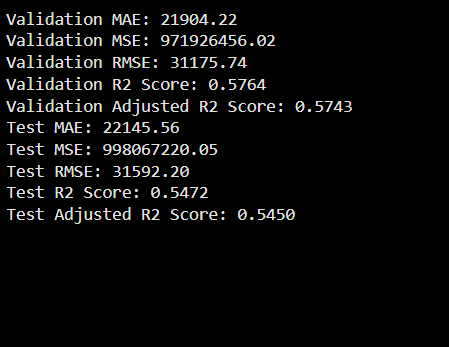
\includegraphics[width=0.5\linewidth]{Output_metrics.png}
    \caption{Performance Metrics }
    \label{fig:distribution}
\end{figure}

\begin{figure}[H]
    \centering
    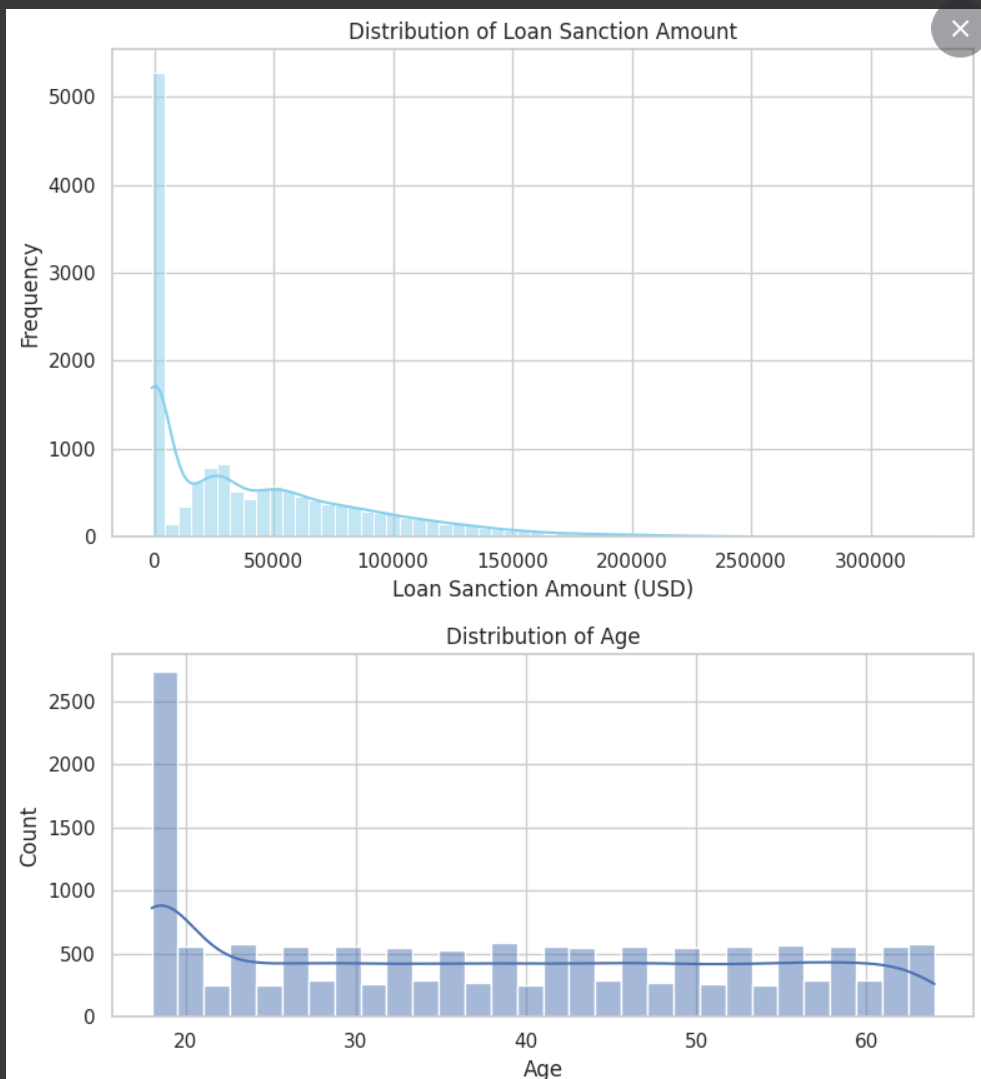
\includegraphics[width=0.5\linewidth]{Distribution.png}
    \caption{Distribution of Dataset}
    \label{fig:distribution}
\end{figure}

\begin{figure}[H]
    \centering
    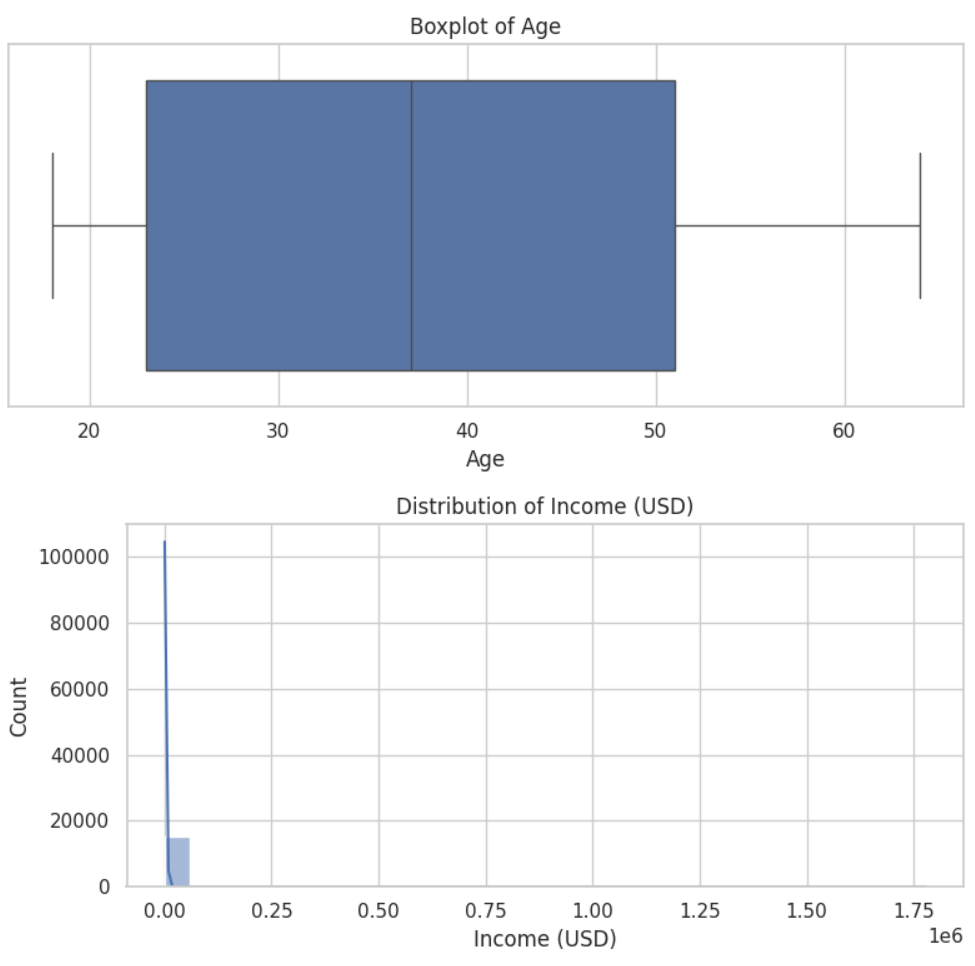
\includegraphics[width=0.5\linewidth]{BoxPlot1.png}
    \caption{Boxplot of Features}
    \label{fig:boxplot}
\end{figure}

\begin{figure}[H]
    \centering
    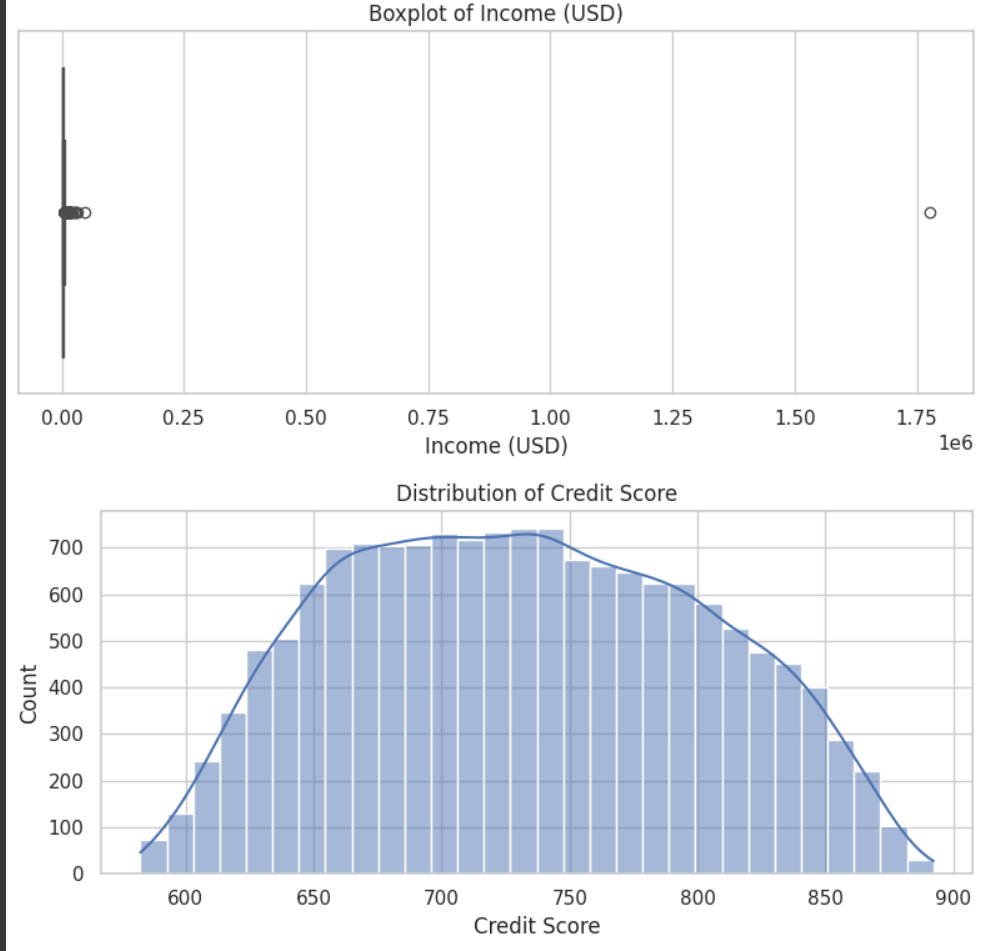
\includegraphics[width=0.5\linewidth]{CreditScore.png}
    \caption{Distribution of Credit Score}
    \label{fig:creditscore}
\end{figure}

\begin{figure}[H]
    \centering
    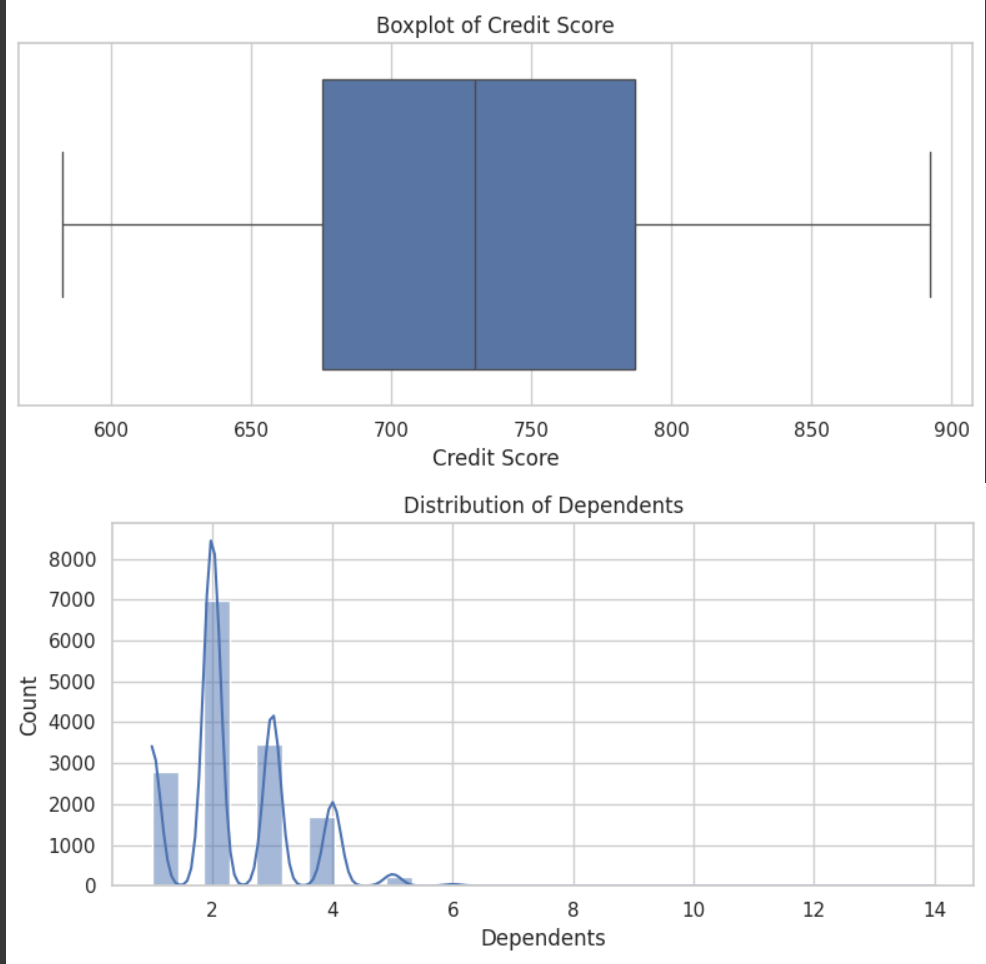
\includegraphics[width=0.5\linewidth]{Dependents.png}
    \caption{Distribution of Dependents}
    \label{fig:dependents}
\end{figure}

\begin{figure}[H]
    \centering
    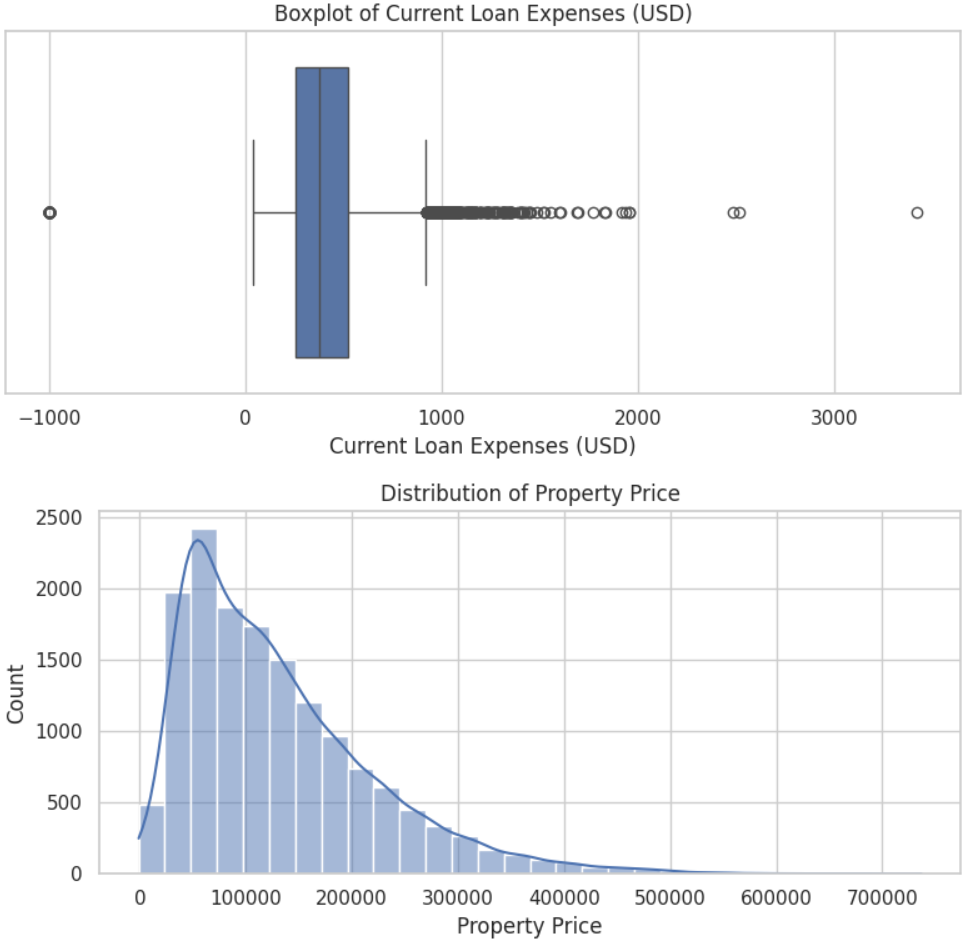
\includegraphics[width=0.5\linewidth]{current_loan.png}
    \caption{Current Loan Expenses Distribution}
    \label{fig:currentloan}
\end{figure}

\begin{figure}[H]
    \centering
    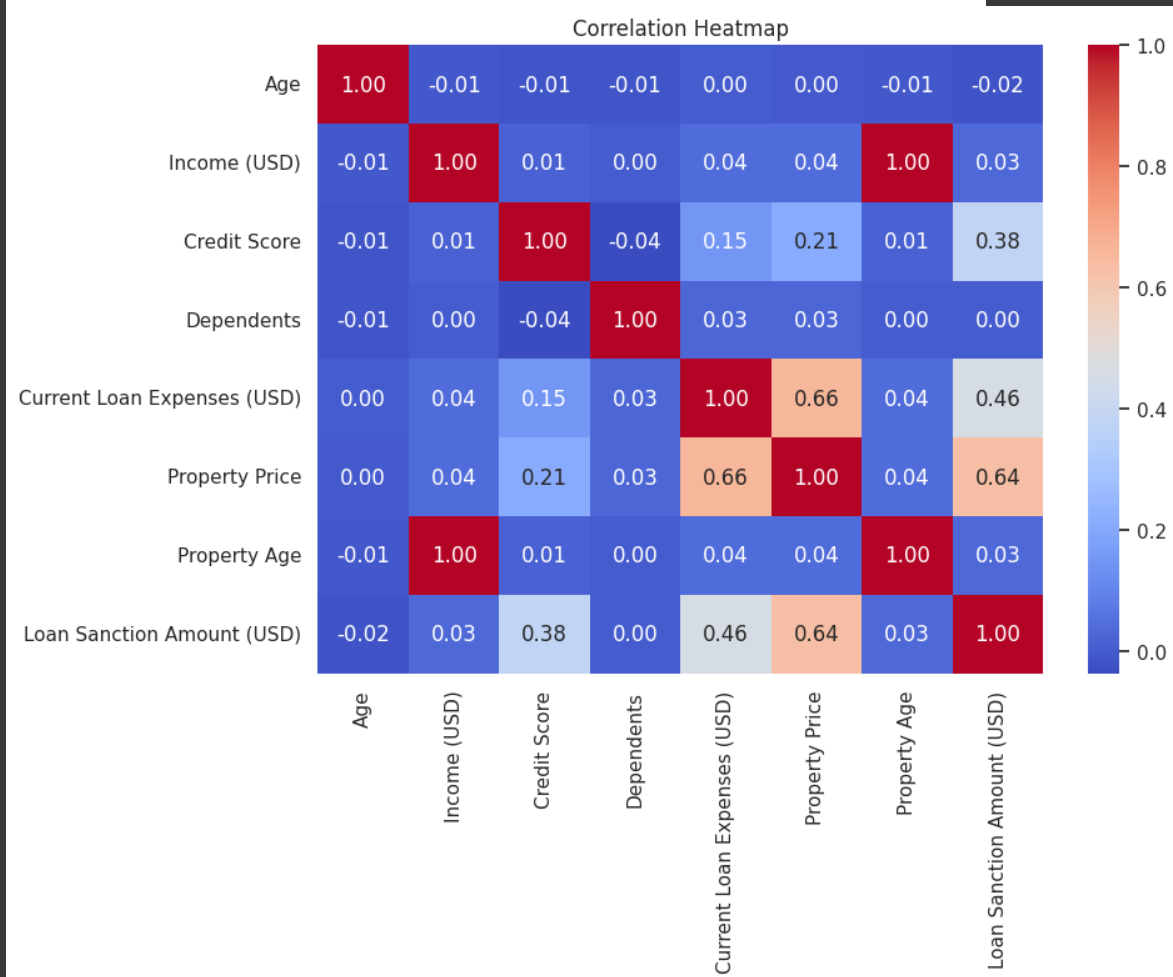
\includegraphics[width=0.5\linewidth]{heatmap.png}
    \caption{Correlation Heatmap}
    \label{fig:heatmap}
\end{figure}

\begin{figure}[H]
    \centering
    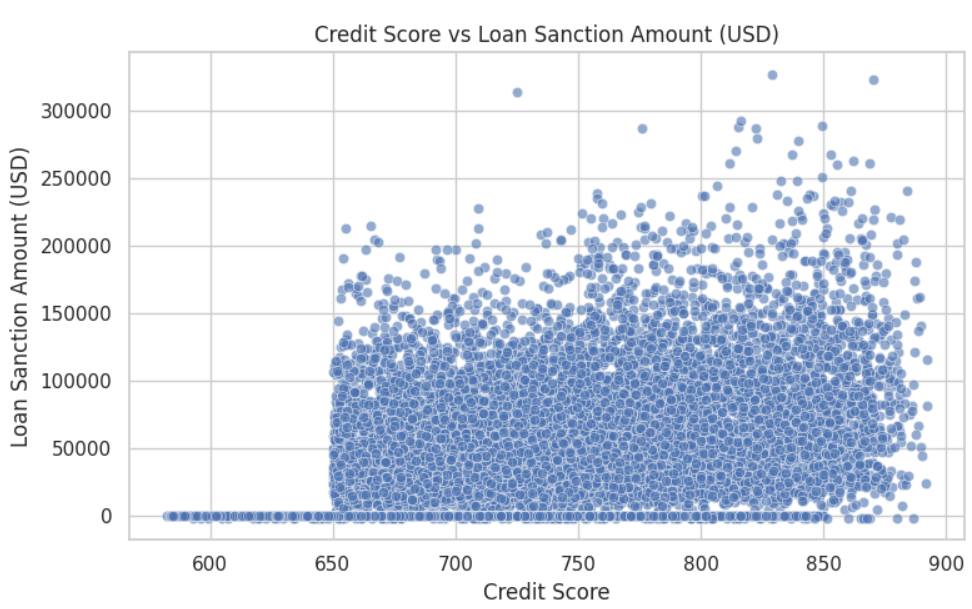
\includegraphics[width=0.8\linewidth]{cs_lmt.png}
    \caption{Credit Score vs Loan Amount}
    \label{fig:cs_lmt}
\end{figure}

\begin{figure}[H]
    \centering
    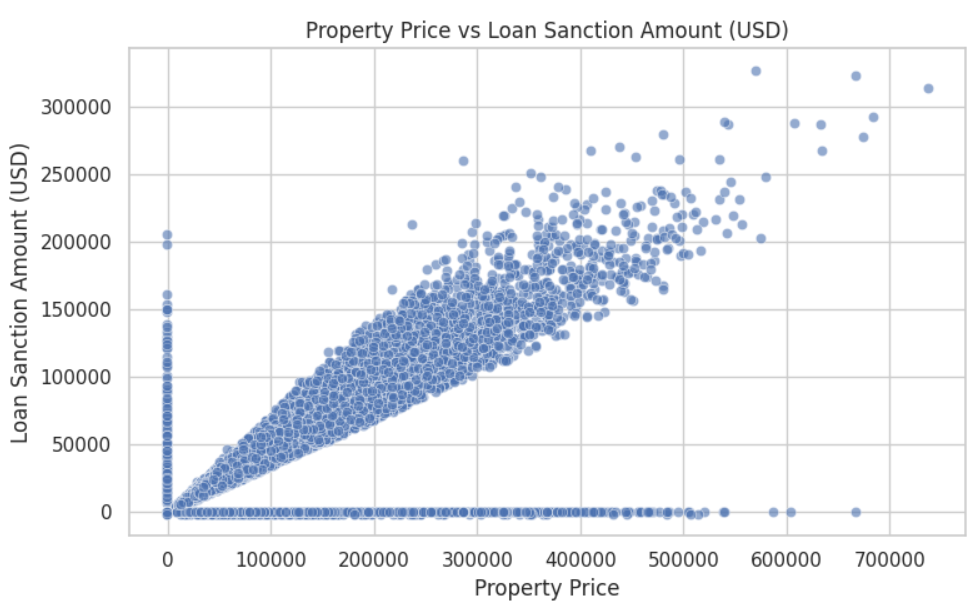
\includegraphics[width=0.8\linewidth]{pt_lmt.png}
    \caption{Property Price vs Loan Amount}
    \label{fig:pt_lmt}
\end{figure}

\begin{figure}[H]
    \centering
    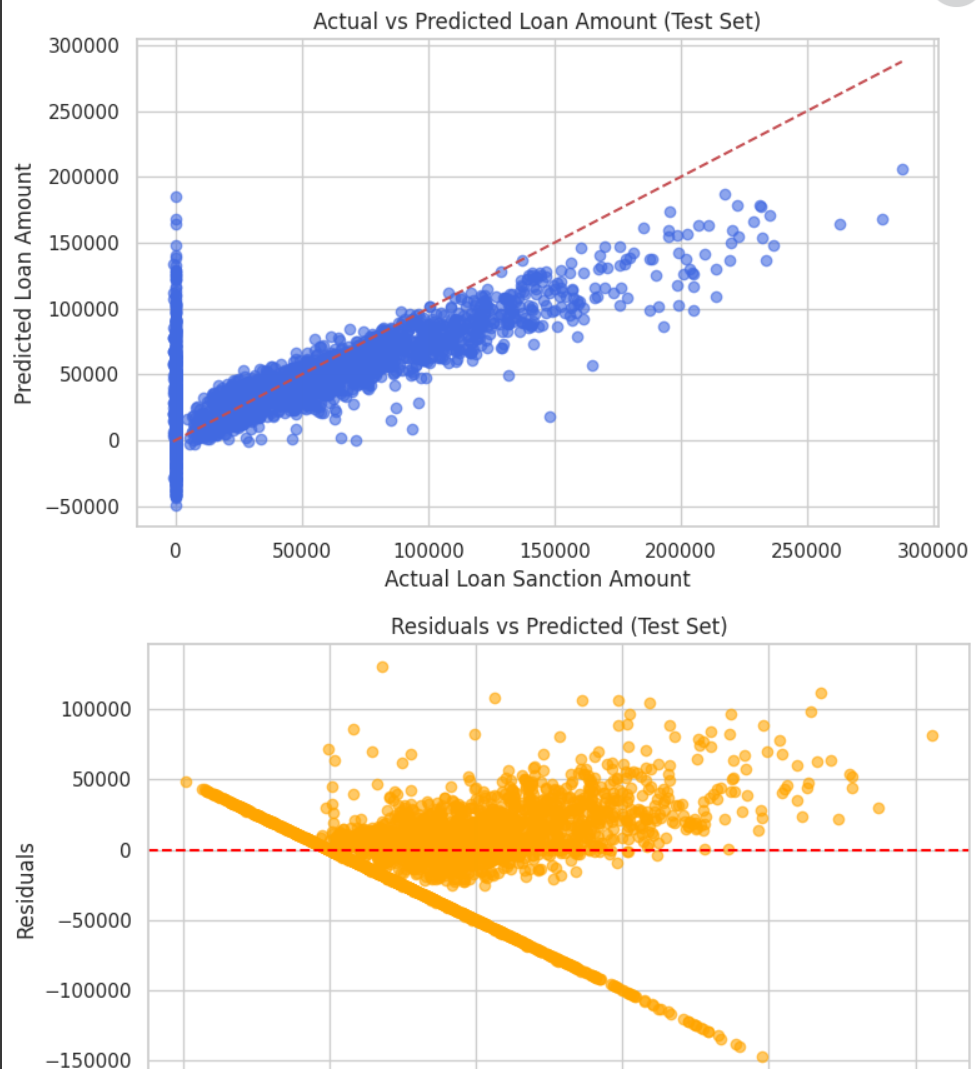
\includegraphics[width=0.8\linewidth]{actual_residual.png}
    \caption{Actual Loan Amount vs Residuals}
    \label{fig:actual_residual}
\end{figure}


\section{Inference Table}

\begin{table}[H]
\centering
\caption{Cross-Validation Results (5-Fold)}
\label{tab:cv_results}
\begin{tabular}{|c|c|c|c|c|}
\hline
\textbf{Fold} & \textbf{MAE} & \textbf{MSE} & \textbf{RMSE} & \textbf{R\textsuperscript{2} Score} \\
\hline
Fold 1 & 22090.85 & $9.96 \times 10^8$ & 31556.51 & 0.5483 \\
Fold 2 & 21386.32 & $9.40 \times 10^8$ & 30655.92 & 0.5652 \\
Fold 3 & 22128.77 & $1.08 \times 10^9$ & 32933.10 & 0.5183 \\
Fold 4 & 21838.68 & $9.65 \times 10^8$ & 31069.29 & 0.5727 \\
Fold 5 & 21917.13 & $9.55 \times 10^8$ & 30896.81 & 0.5817 \\
\hline
\textbf{Average} & \textbf{21872.35} & $\mathbf{9.88 \times 10^8}$ & \textbf{31422.33} & \textbf{0.5572} \\
\hline
\end{tabular}
\end{table}

\vspace{1cm}

\begin{longtable}{|p{5cm}|p{9cm}|}
\caption{Results Summary}
\label{tab:summary} \\
\hline
\textbf{Description} & \textbf{Result} \\
\hline
Dataset Size (after preprocessing) & 15,183 \\
\hline
Train/Test Split Ratio & 60/20/20 (Train/Validation/Test) \\
\hline
Features Used & 
\texttt{['Age', 'Income (USD)', 'Credit Score', 'Dependents', 'Current Loan Expenses (USD)', 'Property Price', 'Property Age', 'Total\_Income', 'Gender', 'Income Stability', 'Profession', 'Type of Employment', 'Has Active Credit Card', 'Co-Applicant', 'Property Type']} \\
\hline
Model Used & Linear Regression \\
\hline
Cross-Validation Used? & Yes \\
\hline
Number of Folds (K) & 5 \\
\hline
Reference to CV Results Table & Table~\ref{tab:cv_results} \\
\hline
MAE on Test Set & 22145.56 \\
\hline
MSE on Test Set & 998067220.05 \\
\hline
RMSE on Test Set & 31592.20 \\
\hline
R\textsuperscript{2} Score on Test Set & 0.5472 \\
\hline
Adjusted R\textsuperscript{2} Score on Test Set & 0.5450 \\
\hline
Most Influential Feature(s) & \texttt{['Co-Applicant\_0', 'Property Price', 'Credit Score']} \\
\hline
Observations from Residual Plot & The residual plot shows a clear pattern with residuals decreasing as predicted values increase, indicating model bias and heteroscedasticity. This suggests the linear model may not fully capture the relationship. \\
\hline
Interpretation of Predicted vs Actual Plot & The plot shows that most predicted values align closely with actual loan amounts along the diagonal line, indicating decent model accuracy. However, there is some spread and underestimation for higher loan amounts, suggesting room for improvement in capturing extreme values. \\
\hline
Any Overfitting or Underfitting Observed? & No significant overfitting or underfitting observed. The training and validation errors are comparable, and residuals do not show extreme patterns, indicating the model generalizes reasonably well. However, some bias at higher values suggests slight underfitting in that range. \\
\hline
\end{longtable}

\section{Best Practices}
\begin{itemize}
    \item \textbf{Data Preprocessing}: Handle missing values carefully (drop or impute), and remove irrelevant columns such as IDs and names that do not contribute to prediction.
    
    \item \textbf{Feature Engineering}: Create new meaningful features (e.g., total income) and apply transformations (e.g., log transformation for skewed data) to improve model performance.
    
    \item \textbf{Scaling and Encoding}: Use scaling (e.g., StandardScaler) for numerical features and one-hot encoding for categorical features to prepare data for linear regression.
    
    \item \textbf{Train-Test Split}: Use proper splits (e.g., 80/20) and consider cross-validation to ensure the model generalizes well and to prevent overfitting.
    
    \item \textbf{Model Evaluation}: Use multiple metrics (MAE, MSE, RMSE, R\textsuperscript{2}) to assess different aspects of model performance.
    
    \item \textbf{Residual Analysis}: Analyze residual plots to detect model bias or heteroscedasticity and decide if further feature engineering or alternative models are needed.
\end{itemize}

\section{Learning Outcomes}
Through this experiment, I have:
\begin{itemize}
    \item Understood the full ML pipeline from data cleaning to model evaluation.
    
    \item Learned the importance of feature engineering and proper data preprocessing.
    
    \item Learned how to visualize data and model results for better insights.
    
    \item Recognized signs of overfitting or underfitting via residual and prediction plots.
    
    \item Used cross-validation for robust model performance assessment.
\end{itemize}


\end{document}
